\documentclass[a4paper,12pt]{article}
%\renewcommand\baselinestretch{1.3}
%\usepackage{times}
\usepackage{setspace}
\usepackage{amsmath}
\usepackage{graphicx}
\usepackage{fancyhdr}

\parskip=7pt
\topmargin=-10mm
%topmargin=15mm
\textheight=250mm
\textwidth=155mm
\oddsidemargin=3mm
\evensidemargin=3mm
\headheight=14.5pt
%headheight=-5pt
\headsep=3mm
%headsep=0mm
%\evensidemargin  \oddsidemargin
%\paperwidth 29.7cm
%\paperheight 21.0cm
\pagestyle{fancy}
\lhead[\it ES431 Astronomy Lab]{\it ES431 Astronomy Lab}
\rhead[\it Odd semester 2012]{\it Odd semester 2012}
\cfoot[\thepage]{\thepage}
\thispagestyle{plain}

\begin{document}
\begin{center}
\Large
{\bf Indian Institute of Space Science and Technology} \\
{\bf Thiruvananthapuram 695 547} \\

\vspace*{5mm}
\Large
\textbf{ES431 $-$ Astronomy Lab} \\
\vspace*{0.5mm}
{\bf Laboratory Evaluation of a CCD camera\footnote{Original notes by Jagadheep, edited by Vikram}} \\
\end{center}

\vspace*{0.2cm}

\large

Charge Coupled Devices (CCDs) are the most common devices used for astronomical imaging. In this laboratory experiment, we will characterize the KAF0401E CCD in the SBIG ST-7XE camera. The device has $765 \times 510$ pixels with a pixel size of $9 \times 9~\mu$m, the overall size of the array being $6.9 \times 4.6$~mm.

The basic operating principles of CCDs are described in ``Astrophysical Techniques'' by C.~R.~Kitchin, pp. 24$-$31. The first step is generation of charges by incident photons through the photoelectric effect. The charges are collected by potential wells created by an array of electrodes called gates on the CCD. The collected charge is then transferred in a manner analogous to a conveyor belt (see Figure 1) to an on-chip amplifier followed by conversion of charges to output voltages which can be amplified off-chip, converted to a digital signal, and recorded on computer.

\begin{figure}[!htb]
\centering
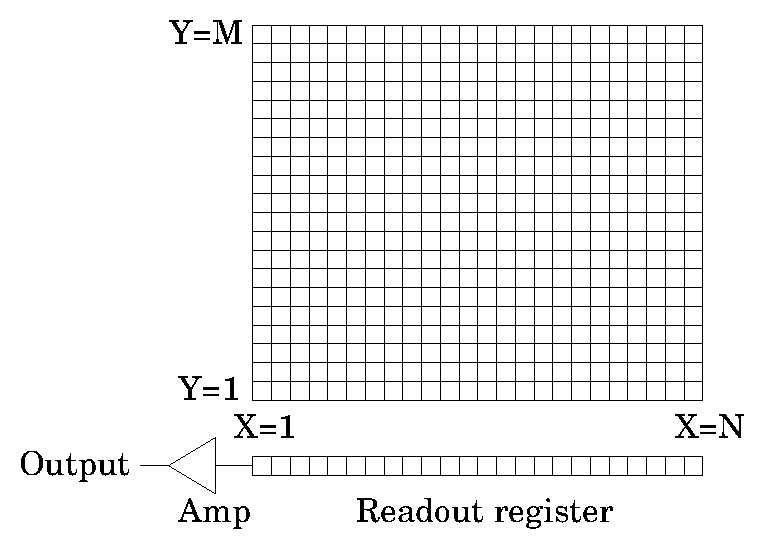
\includegraphics[width=0.6\textwidth]{CCD.eps}
\caption{Schematic of a CCD showing the pixels and the readout mechanism.}
\end{figure}

The charge transfer is a two-step process. First, a row is shifted to the Y=0 position (called a parallel transfer). Next, all the charges in the row are transferred sequentially to the X=0 position and read out (called a serial transfer). The electromechanical shutter covers the CCD during the readout to prevent streaking across the image. Hence, a new exposure cannot be started before the previous image is read out.

The CCD is cooled with a solid state thermoelectric cooler. The cooler transfers heat out of the CCD and dissipates it into a heat sink, which is part of the mechanical housing. This heat is then dumped into the air using a heat exchanger and a small fan. The efficiency of the cooling (and hence the lowest operating temperature) depends on the ambient temperature.


\noindent {\bf \Large Getting Started:}

First connect the the USB cable to the portable computer (operating system should be Windows). Then connect power lines to the camera and switch the power on (there is a switch in the adapter). The CCD operating software, CCDOPS can now be started. Click on ``Establish Comm Link'' to establish a communication link between the computer and the camera. Once the COM link is established, click on ``Camera Setup'' (or Ctrl-U), and choose a setpoint temperature. Once you type in the setpoint, set the temperature control to active, and hit ENTER. Watch the temperature (the quantity displayed as a percentage is the cooling efficiency) on the bottom right, and wait until the setpoint temperature is reached.

To take an exposure, click on the ``Grab'' icon. Type in the exposure time (units are seconds), select whether to take an exposure, dark frame or both, and then click OK. Once the exposure is completed, the CCD is read and the image is shown on the screen. To save the image, click on ``File'' and select ``Save''. Choose the format to save the image (you should use FITS format), type in the filename (using meaningful filenames which have information on the nature of exposure and exposure time can save effort later) after selecting a suitable directory, and then click OK.

\noindent {\bf \Large CCD characterization:}

Note that there can be fixed pattern noise in a chip, for example from hot and dead pixels. To remove this, you should always take a bias frame (taken with exposure time of zero; in this case, this will default to the minimum exposure time of 0.12~s). In any analysis, you should subtract the bias frame from the image under consideration, and only then should you measure any parameters.

\begin{enumerate}
{\bf \item Read Noise:} In the absence of a photon signal, even if the chip is cooled to a low enough temperature that there are no thermally generated charges, there is still noise in the system. This comes from the various electronic components. This read noise is the ultimate noise floor for the device. 

To measure the read noise, put the lens cap on the CCD camera to prevent any light from entering the camera. Then take a 1~second exposure. Measure the rms in several regions of the image. Repeat the procedure on several exposures (you should take at least 5 exposures with the same exposure time). Do the same measurement with a 3~second and 0.5~second exposure time and check if there is any dependence of read noise on the exposure time.

{\bf \item Dark Current:} In the absence of a photon signal, the potential wells of a CCD can collect thermally generated charges in the solid state material. This gives rise to dark current. The dark current is a signal that is proportional to the exposure time. In addition, it is close to a shot noise process. Hence, you will also see a fluctuation in the number of dark current charges that is in accordance with Poisson statistics -- i.e. if the number of electrons from dark current is $N_d$, the uncertainty is $\sqrt{N_d}$. The dark current signal can be subtracted from the measured signal in an observation of a science target. However, the fluctuations in the dark current signal is a noise term that cannot be corrected for.

To measure the dark current, there are two methods. You can either take exposures with the lens cap on, or you can take a dark frame (using the options in the ``Grab'' dialog). You should make measurements using both methods and compare results. You should interpret the result if the measurements do not give the same values. First take a bias frame. Then, take longer and longer exposures (e.g. 1~s, 2~s, 5~s, 10~s, etc.) until around 500~seconds. Measure the mean signal in each exposure and plot it as a function of time. The slope of the curve will give the dark current. Over the course of your exposures, you should take several bias frames to check whether the bias level is fluctuating or not.

The next step is to measure the dark current as a function of temperature. Choose an exposure time that will give you a reliable estimate of the dark current (if you choose too short an exposure time, you will be dominated by read noise; if you choose too long an exposure time, you will end up spending a lot of time making the measurements). Set the operating temperature of the CCD through the camera setup dialog, and wait until the temperature is stable. Then, take a bias frame and a dark frame with the chosen exposure time. Repeat the procedure for different operating temperatures. You should have data for temperatures of 20, 15, 10, 5, 0, $-$5, and if possible $-$10$^\circ$~C. Plot the dark current as a function of temperature.

{\bf \item Linearity:} Is the signal reported from the read-out of the CCD proportional to the number of photons hitting the CCD? This can be tested by exposing the CCD for increasingly long times to a constant intensity and plotting the reported data numbers as a function of time. 

The object is to make a series of exposures which result in a wide range of data number values from a few hundred to 60,000. It is important to ensure that the light level stays constant throughout the exposures. For this purpose, you will use a setup where light from a set of LEDs powered by a 9~V battery is diffused through an aperture and a sheet of paper. Cover the entire setup with black cloth so that stray light, which can saturate the camera quickly, can be avoided. First measure the data count for an exposure time of say 5~seconds. Use this to determine the exposure times to get data numbers from a few hundred to 60,000. Note that the shutter may not be reliable at very low exposure times. Also, the camera may not offer linear operation at high operating temperatures. Hence, carry out this experiment keeping the operating temperature at $5^\circ$~C or lower.

{\bf \item Conversion from data numbers to number of electrons:} The signal in the potential wells of the CCD are in units of number of electrons, that are related to the incident number of photons multiplied by the quantum efficiency. The signal reported by the readout electronics is in data numbers. Let the conversion factor between data numbers and number of electrons be $K$. Now, in accordance with the shot noise statistics, if the signal comprises of $N_e$ electrons, the noise (assuming that it is well above read noise) is $\sqrt{N_e}$. Thus, in terms of data number, the signal is $KN_e$, and the noise is $K\sqrt{N_e}$. Thus, $K$ can be determined by plotting the square of noise as a function of the signal. Alternatively, the intercept of the plot of $\log_{10}(\mathrm{noise})$ as a function of $\log_{10}(\mathrm{signal})$ gives $\log_{10}K$. Use the data obtained previously to measure the conversion factor $K$.

{\bf \item Blooming:} If the CCD is exposed to a very bright source (e.g. a star), the potential wells in the image will be filled beyond their capacity. The excess charges will spill over into adjacent wells and the image size will expand. During the read-out process, a small percentage of the charge from the full wells gets left behind and forms a trail behind the image. In extreme cases, this trail will extend both in the vertical and horizontal directions. These effects are called blooming. Note that the ``X'' shaped spikes that are seen in astronomical images of bright objects are due to diffraction by the supports of the telescope's secondary mirror and are not related to blooming.

To check the blooming performance of the chip, you need to first take an image of a ``point source'' that does not saturate the well at its core. Next, increase the length of exposure (by a factor of two or so each time) until the image of the point source begins to bleed across the image. By what factor has the exposure exceeded the exposure needed to reach saturation (data number of 65,000)? The direction of the bleeding indicates the direction in which charge is flowing as it is read out. Keep a note of this direction.

{\bf \item Charge Transfer Efficiency:} To measure the charge transfer efficiency, one needs to understand it in an operational sense. Let us assume that the read-out is in the left to right direction.  Moreover, let there be $N$ electrons in a certain pixel and zero in all the others in the row. Also, let $\alpha$ be the charge transfer efficiency and $\epsilon = 1-\alpha$. Then, the charges in the individual pixels in the beginning and each successive read look like the following:
\begin{tabular*}{0.7\textwidth}{@{\extracolsep{\fill}}ccccccc}
$N$ & 0 & 0 & 0 & 0 & 0 & $\ldots$ \\
$N\epsilon$ & $N\alpha$ & 0 & 0 & 0 & 0 & $\ldots$ \\
$N\epsilon^2$ & $2N\epsilon\alpha$ & $N\alpha^2$ & 0 & 0 & 0 & $\ldots$ \\
$N\epsilon^3$ & $3N\epsilon^2\alpha$ & $3N\epsilon\alpha^2$ & $N\alpha^3$ & 0 & 0 & $\ldots$ 
\end{tabular*}

The pattern should remind you of the binomial expansion from which you can generalize to $P$ transfers. 

How do you get electrons only in one pixel to start with? Cosmic rays provide the answer. Cosmic rays strike one or a few adjacent pixels and deposit several to many thousand electrons in them. If the charge transfer efficiency is not perfect, the cosmic rays will blur out as the charge is transferred across the chip. Analyze one of the dark frames with many cosmic ray hits to get the charge transfer efficiency. Do your analysis for several cosmic ray hits (at least five). Keep in mind that some of the initial cosmic ray charge may have actually gone into several pixels including the pixel which is trailing the main hit. Hence, your derived values will be a {\it lower limit} to the actual charge transfer efficiency.

\end{enumerate}

\noindent {\bf \Large Shutting down:}

To shut down the camera, select ``Shutdown'' in the ``Camera'' menu. This triggers an internal warm-up procedure in the camera, preventing rapid warming of the CCD chip. The chip is not likely to be harmed if it warms up suddenly, for example in a power failure. However, slow warm-up places less stress on the chip.

Before you shut down the computer, copy your files onto a memory stick! You will be analyzing the data using IRAF in a different machine.

\noindent {\bf \Large The report:}

You will be taking the measurements with the CCD in groups of two. However, each person should analyze the data in IRAF independently. Different groups will be given different operating temperatures. So, don't try to reproduce or copy results of other groups! For all quantities, you should quote results with uncertainties. The precision with which you quote your result must depend on the uncertainty. For instance, if the uncertainty is in the first decimal (say, 0.2), it makes no sense to quote a parameter beyond the first decimal place (such as 3.217939) -- the result should be $3.2 \pm 0.2$. Your report should include \underline{\it brief} information on how you achieved your result, such as the number of exposures along with their exposure times, data analysis procedure used in IRAF, etc.

\end{document}
